\documentclass{ximera}

\newcommand{\RR}{\mathbb R}
\renewcommand{\d}{\,d}
\newcommand{\dd}[2][]{\frac{d #1}{d #2}}
\renewcommand{\l}{\ell}
\newcommand{\ddx}{\frac{d}{dx}}
\newcommand{\dfn}{\textbf}
\newcommand{\eval}[1]{\bigg[ #1 \bigg]}


\outcome{Find the critical points of a function of two variables.}
\outcome{Use the second derivative test to classify local extrema.}
\outcome{Find local extrema of functions of two variables.}



\title[Dig-In:]{Maxima and minima}

\begin{document}
\begin{abstract}
  We see how to find extrema of functions of several variables.
\end{abstract}
\maketitle


Given a function $z=F(x,y)$, we are often interested in points where
$z$ takes on the largest or smallest values. For instance, if $z$
represents a cost function, we would likely want to know what $(x,y)$
values minimize the cost. If $z$ represents the ratio of a volume to
surface area, we would likely want to know where $z$ is greatest. This
leads to the following definition that we will state rather generally,
but use mostly in the case of a function $F:\R^2\to\R$.

\begin{definition}
Let $F:\R^n\to\R$ be defined on a set $S\subset\R^n$ containing the
point $\vec{c}$ in $\R^n$.
\index{maximum!local}\index{minimum!local}\index{extrema!absolute}\index{maximum!absolute}\index{minimum!absolute}
\begin{itemize}
\item If there is an open disk $B$ containing $\vec{c}$ such that
  $F(\vec{c}) \geq F(\vec{x})$ for all $\vec{x}$ in $B$, then $F$ has a
  \dfn{local maximum} at $\vec{c}$; if $F(\vec{c}) \leq F(\vec{x})$ for all
  $\vec{x}$ in $B$, then $F$ has a \dfn{local minimum} at $\vec{c}$.
\item If $F(\vec{c})\geq F(\vec{x})$ for all $\vec{x}$ in $S$, then $F$ has
  an \dfn{absolute maximum} at $\vec{c}$; if $F(\vec{c})\leq F(\vec{x})$ for
  all $\vec{x}$ in $S$, then $F$ has an \dfn{absolute minimum} at
  $\vec{c}$.
\item If $F$ has a local maximum or minimum at $\vec{c}$, then $F$ has a
  \dfn{local extrema} at $\vec{c}$; if $F$ has an absolute maximum or
  minimum at $\vec{c}$, then $F$ has a \dfn{absolute extrema} at $\vec{c}$.
\end{itemize}
\end{definition}


\section{Critical points}



If $F$ has a local or absolute maximum at $\vec{c}$, it means the
gradient will point ``nowhere'' since the gradient points in the
initial direction of greatest increase. This means it is pointing in a
``direction'' whose components are either zero or undefined. In an
entirely similar way, the gradient will be a vector whose components
are either zero or undefined at local minimums as well. 

\begin{definition}
  Let $z = F(x,y)$ be continuous on an open set $S$. A
  \dfn{critical point} $\vec{c}=\vector{c_1,c_2}$ of $F$ is a point in $S$ such
  that
  \begin{itemize}
  \item $\grad F(\vec{c}) = \vec{0}$ or
  \item $\grad F(\vec{c})$ is undefined.
  \end{itemize}
\end{definition}

\begin{theorem}
Let $F:\R^n\to\R$ be defined on an open set $S$ containing
$\vec{c}$. If $F$ has a local extrema at $\vec{c}$, then $\vec{c}$ is a
critical point of $F$.
\end{theorem}

Therefore, to find local extrema, we find the critical points of $F$
and determine which correspond to local maxima, local minima, or
neither. We'll use examples to demonstrate this process.

\begin{example}
  Let $F(x,y) = x^2+y^2-xy-x-2$. Find the local extrema of $F$.
  \begin{explanation}
    We start by computing $\grad F$:
    \[
    \grad F(x,y) = \vector{\answer[given]{2x-y-1},\answer[given]{2y-x}}
    \]
    Each component of $\grad F$ is never undefined. A critical point
    occurs when $\grad F(x,y) = \vec{0}$, leading us to solve the
    following system of linear equations:
    \[
    2x-y-1 =\answer[given]{0}\quad \text{and}\quad -x+2y = \answer[given]{0}.
    \]
    This solution to this system is $x=\answer[given]{2/3}$,
    $y=\answer[given]{1/3}$. So the critical point is
    $\vec{c}=\vector{\answer[given]{2/3},\answer[given]{1/3}}$. When
    possible, it is good to confirm your answer with a graph:
    \begin{image}
      \begin{tikzpicture}
        \begin{axis}%
          [tick label style={font=\scriptsize},axis on top,
	    axis lines=center,
	    view={135}{25},
	    name=myplot,
	    %xtick=\empty,
	    %ytick={5},
	    %ztick={.7,-.7},
	    minor xtick=1,
	    minor ytick=1,
	    ymin=-1.5,ymax=2.5,
	    xmin=-1.5,xmax=2.5,
	    zmin=-2.5, zmax=5.5,
	    every axis x label/.style={at={(axis cs:\pgfkeysvalueof{/pgfplots/xmax},0,0)},xshift=-5pt,yshift=-1pt},
	    xlabel={\scriptsize $x$},
	    every axis y label/.style={at={(axis cs:0,\pgfkeysvalueof{/pgfplots/ymax},0)},xshift=4pt,yshift=-4pt},
	    ylabel={\scriptsize $y$},
	    every axis z label/.style={at={(axis cs:0,0,\pgfkeysvalueof{/pgfplots/zmax})},xshift=0pt,yshift=4pt},
	    zlabel={\scriptsize $z$},colormap/cool
	  ]
          
          \addplot3[domain=-1.:3,,y domain=-1.:3,mesh,samples y=10,very thin,z buffer=sort] {x^2+y^2-x*y-x-2};
          
          \addplot3 [ultra thick,penColor, smooth,domain=-1.:3,samples=20,samples y=0,opacity=.3] ({x},{3},{x^2+3^2-x*3-x-2});

          \addplot3 [ultra thick,penColor, smooth,domain=-1.:3,samples=20,samples y=0,opacity=.3] ({x},{-1},{x^2+(-1)^2-x*(-1)-x-2});

          \addplot3 [ultra thick,penColor, smooth,domain=-1.:3,samples=20,samples y=0,opacity=.3] ({-1},{x},{x^2+(-1)^2-x*(-1)-(-1)-2});

          \addplot3 [ultra thick,penColor, smooth,domain=-1.:3,samples=20,samples y=0,opacity=.3] ({3},{x},{x^2+3^2-x*3-3-2});

          \filldraw [black,opacity=.7] (axis cs:.666,.333,-2.333) circle (3pt);
          \node[right] at (axis cs:2/3,1/3,-7/3) {$(2/3,1/3,-7/3)$};
        \end{axis}
      \end{tikzpicture}
    \end{image}
    The graph above shows $F$ along with this critical point. It is
    clear from the graph that this is a local minimum.
  \end{explanation}
\end{example}

\begin{example}
  Let $F(x,y) = -\sqrt{x^2+y^2}+2$. Find the local extrema of $F$.
  \begin{explanation}
    We start by computing $\grad F$:
    \[
    \grad F(x,y) = \vector{\frac{-x}{\sqrt{x^2+y^2}},\frac{-y}{\sqrt{x^2+y^2}}}
    \]
    Here the only critical point is at $\vector{0,0}$ because $\grad
    F$ is undefined at $\vector{0,0}$. 
    \begin{image}
      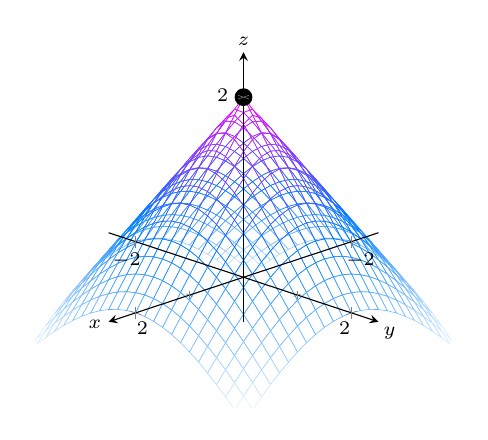
\begin{tikzpicture}
        \begin{axis}%
          [tick label style={font=\scriptsize},axis on top,
	    axis lines=center,
	    view={135}{25},
	    name=myplot,
	    %xtick=\empty,
	    %ytick={5},
	    %ztick={.7,-.7},
	    minor xtick=1,
	    minor ytick=1,
	    ymin=-2.5,ymax=2.5,
	    xmin=-2.5,xmax=2.5,
	    zmin=-0.5, zmax=2.5,
	    every axis x label/.style={at={(axis cs:\pgfkeysvalueof{/pgfplots/xmax},0,0)},xshift=-5pt,yshift=-1pt},
	    xlabel={\scriptsize $x$},
	    every axis y label/.style={at={(axis cs:0,\pgfkeysvalueof{/pgfplots/ymax},0)},xshift=4pt,yshift=-4pt},
	    ylabel={\scriptsize $y$},
	    every axis z label/.style={at={(axis cs:0,0,\pgfkeysvalueof{/pgfplots/zmax})},xshift=0pt,yshift=4pt},
	    zlabel={\scriptsize $z$},colormap/cool
	  ]
          
          \addplot3[domain=-2:2,,y domain=-2:2,mesh,samples=25,samples y=25,very thin,z buffer=sort] {-sqrt(x^2+y^2)+2};
          \filldraw [black,] (axis cs:0,0,2) circle (3pt);
        \end{axis}
      \end{tikzpicture}
    \end{image}
    The surface of $F$ is graphed above along with the point
    $(0,0,2)$. The graph shows that this point is the absolute maximum
    of $F$.
  \end{explanation}
\end{example}

In each of the previous two examples, we found a critical point of $F$
and then determined whether or not it was a local (or absolute)
maximum or minimum by graphing. It would be nice to be able to
determine whether a critical point corresponded to a max or a min
without a graph. Before we develop such a test, we do one more example
that sheds more light on the issues our test needs to consider.


\begin{example}
  Let $F(x,y) = x^3-3x-y^2+4y$. Find the local extrema of $F$.
  \begin{explanation}
    Once again we start by computing $\grad F$:
    \[
    \grad F(x,y) = \vector{\answer[given]{3x^2-3},\answer[given]{-2y+4}}
    \]
    Each component is always defined. Setting $\grad F(x,y) = \vec{0}$
    and solving for $x$ and $y$, we find
    \begin{align*}
      x &=\pm \answer[given]{1}\\
      y &= \answer[given]{2}.
    \end{align*}
    We have two critical points: $\vector{-1,2}$ and $\vector{1,2}$. To determine
    if they correspond to a local maximum or minimum, we consider the
    graph of $F$ below:
    \begin{image}
      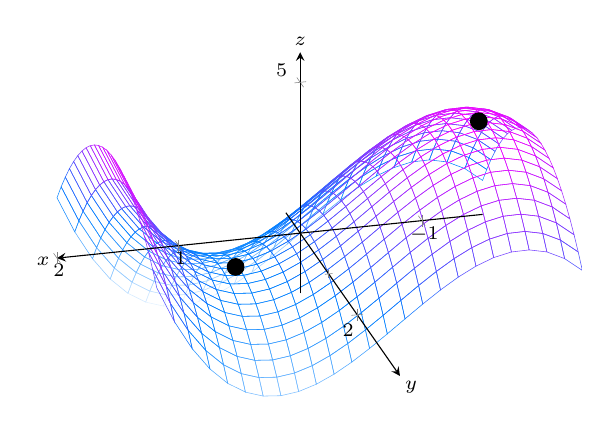
\begin{tikzpicture}
        \begin{axis}%
          [tick label style={font=\scriptsize},axis on top,
	    axis lines=center,
	    view={165}{35},
	    name=myplot,
	    %xtick=\empty,
	    %ytick={5},
	    %ztick={.7,-.7},
	    minor xtick=1,
	    minor ytick=1,
	    ymin=-.5,ymax=3.5,
	    xmin=-1.5,xmax=2,
	    zmin=-2, zmax=6,
	    every axis x label/.style={at={(axis cs:\pgfkeysvalueof{/pgfplots/xmax},0,0)},xshift=-5pt,yshift=-1pt},
	    xlabel={\scriptsize $x$},
	    every axis y label/.style={at={(axis cs:0,\pgfkeysvalueof{/pgfplots/ymax},0)},xshift=4pt,yshift=-4pt},
	    ylabel={\scriptsize $y$},
	    every axis z label/.style={at={(axis cs:0,0,\pgfkeysvalueof{/pgfplots/zmax})},xshift=0pt,yshift=4pt},
	    zlabel={\scriptsize $z$},colormap/cool
	  ]
          \addplot3[domain=-1.5:2,,y domain=-0:3.5,mesh,samples=25,samples y=25,very thin,z buffer=sort] {x^3-3*x-y^2+4*y};

          \filldraw [black,] (axis cs:1,2,2) circle (3pt);
          \filldraw [black,] (axis cs:-1,2,6) circle (3pt);
        \end{axis}
      \end{tikzpicture}
    \end{image}

    %% in Figure \ref{fig:multi_extreme3}.
    %% \mfigure[scale=1.1]{.7}{The surface in Example
    %%   \ref{ex_multi_extreme3} with both critical points
    %%   marked.}{fig:multi_extreme3}{figures/figmulti_extreme3}

    The critical point $\vector{-1,2}$ clearly corresponds to a local
    maximum. However, the critical point at $\vector{1,2}$ is neither
    a maximum nor a minimum, displaying a different, interesting
    characteristic.

    If one walks parallel to the $y$-axis towards this critical point,
    then this point becomes a local maximum along this path. But if
    one walks towards this point parallel to the $x$-axis, this point
    becomes a local minimum along this path. A point that seems to act
    as both a max and a min is a \textit{saddle point}. A formal
    definition follows.
  \end{explanation}
\end{example}


\begin{definition}
  Let $F:\R^n\to\R$ and $\vec{c}$ be in the domain of $F$ where $\grad
  F(\vec{c})=\vec{0}$ at $\vec{c}$. The point $\vec{c}$ is a
  \dfn{saddle point} of $F$ if, for every open disk $B$ containing
  $\vec{c}$, there are points $\vec{a}_1$ and $\vec{a}_2$ in $B$ such
  that $F(\vec{c})>F(\vec{a}_1)$ and $F(\vec{c})<F(\vec{a}_2)$.
\end{definition}

The most obvious example of a saddle point is a the point determined
by $\vector{0,0}$ on a hyperbolic paraboloid of the form $z = \pm x^2 \mp y^2$. 
\begin{image}
  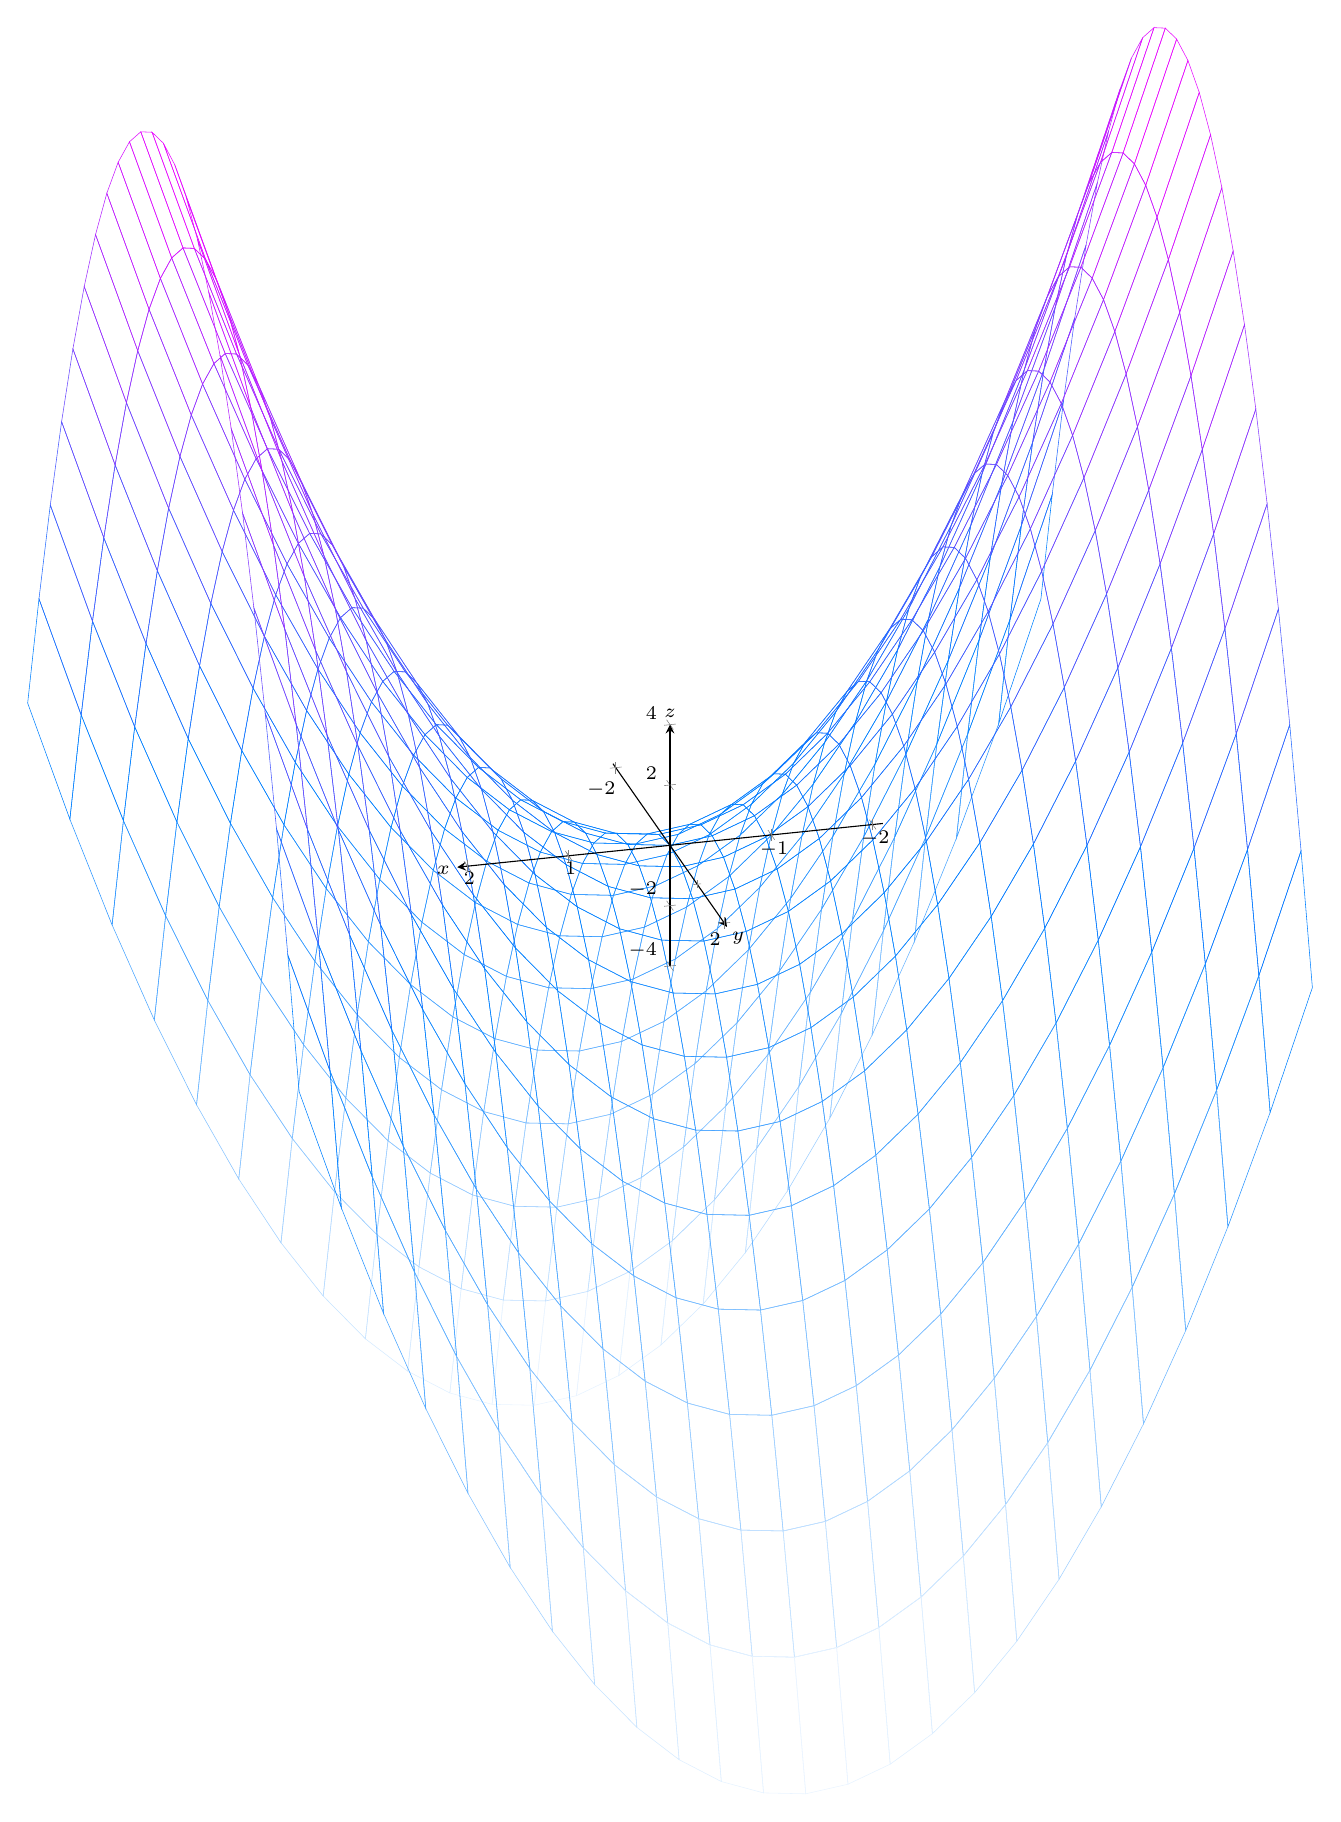
\begin{tikzpicture}
    \begin{axis}%
      [tick label style={font=\scriptsize},axis on top,
	axis lines=center,
	view={165}{35},
	name=myplot,
	%xtick=\empty,
	%ytick={5},
	%ztick={.7,-.7},
	minor xtick=1,
	minor ytick=1,
	ymin=-2.1,ymax=2.1,
	xmin=-2.1,xmax=2.1,
	zmin=-4, zmax=4,
	every axis x label/.style={at={(axis cs:\pgfkeysvalueof{/pgfplots/xmax},0,0)},xshift=-5pt,yshift=-1pt},
	xlabel={\scriptsize $x$},
	every axis y label/.style={at={(axis cs:0,\pgfkeysvalueof{/pgfplots/ymax},0)},xshift=4pt,yshift=-4pt},
	ylabel={\scriptsize $y$},
	every axis z label/.style={at={(axis cs:0,0,\pgfkeysvalueof{/pgfplots/zmax})},xshift=0pt,yshift=4pt},
	zlabel={\scriptsize $z$},colormap/cool,clip=false
      ]
      \addplot3[mesh,samples=25,samples y=25,very thin,z buffer=sort] {x^2-y^2};
    \end{axis}
      \end{tikzpicture}
\end{image}

When thinking about a graph of $z= F(x,y)$ at a saddle point, the
instantaneous rate of change in all directions is $0$ and there are
points nearby with $z$-values both less than and greater than the
$z$-value of the saddle point.



\section{The second derivative test}

In theory to identify local extrema verses saddle points, we could
compute the Taylor polynomial of degree $2$ at the critical point in
question, and then identify the Taylor polynomial as either:
\begin{description}
\item[Elliptic paraboloid] Indicating we have found local extrema.
\item[Hyperbolic paraboloid] Indicating that we are at a saddle point.
\end{description}
Fortunately, as we have seen, there is a second derivative test that
does exactly this for us. We will now restate this test in the context
of identifying local extrema.

\begin{theorem}[Second derivative test]
  Given a function $F:\R^2\to \R$, and a critical point $\vec{c}$ where
  \[
  D(\vec{c}) = F^{(2,0)}(\vec{c})F^{(0,2)}(\vec{c})-F^{(1,1)}(\vec{c})^2.
  \]
  \begin{itemize}
  \item If $D(\vec{c})>0$ and $F^{(2,0)}(\vec{c})<0$ then $\vec{c}$ is a local maximum.
  \item If $D(\vec{c})>0$ and $F^{(2,0)}(\vec{c})>0$ then $\vec{c}$ is a local minimum.
  \item	If $D(\vec{c})<0$, then $\vec{c}$ is a saddle point.
  \item If $D(\vec{c})=0$, the test is inconclusive.
  \end{itemize}
\end{theorem}

We first practice using this test with the function in the previous
example, where we visually determined we had a local maximum and a
saddle point.

\begin{example}
  Let $F(x,y) = x^3-3x-y^2+4y$. Determine whether the function has a
  local minimum, maximum, or saddle point at each critical point.
  \begin{explanation}
    We determined previously that the critical points of $F$ are
    $\vector{-1,2}$ and $\vector{1,2}$. To use the second derivative
    test, we must find the second partial derivatives of $F$:
    \begin{align*}
      F^{(2,0)}(x,y) &= \answer[given]{6x}\\
      F^{(0,2)}(x,y) &= \answer[given]{-2}\\
      F^{(1,1)}(x,y) &= \answer[given]{0}
    \end{align*}
    Thus:
    \[
    D(x,y) = \answer[given]{-12x}
    \]
    Since $D(-1,2) = \answer[given]{12}>0$, and $F^{(2,0)}(-1,2) =
    \answer[given]{-6}$, by the second derivative test, locally looks
    like \wordChoice{\choice[correct]{an elliptic paraboloid}\choice{a hyperbolic paraboloid}} at $\vector{-1,2}$, meaning $F$ has a
    local maximum at $\vector{-1,2}$.
    
    Since $D(1,2) = \answer[given]{-12} <0$, by the second derivative
    test, $F$ locally looks like \wordChoice{\choice{an elliptic paraboloid}\choice[correct]{a hyperbolic paraboloid}} at
    $\vector{-1,2}$ meaning $F$ has a saddle point at $\vector{1,2}$.
    
    The second derivative test has confirmed the visual evidence we
    found before.
  \end{explanation}
\end{example}

\begin{example}
  Find the local extrema of $F(x,y) = x^2y+y^2+xy$.
  \begin{explanation}
    We start by finding the first and second partial derivatives of $F$:
    \begin{align*}
      F^{(1,0)}(x,y) &= 2xy+y\\
      F^{(0,1)}(x,y) &= x^2+2y+x \\
      F^{(2,0)}(x,y) &= 2y\\
      F^{(0,2)}(x,y) &= 2\\
      F^{(1,1)}(x,y) &= 2x+1 
    \end{align*}
    We find the critical points by finding where $\grad F(x,y) =
    \vec{0}$, since the partial derivatives are defined everywhere on
    $\R^2$. With a bit of algebra we can show that there are three
    critical points
    \begin{itemize}
    \item $\vector{0,0}$,
    \item $\vector{\answer[given]{-1},0}$, and
    \item $\vector{\answer[given]{-1/2},\answer[given]{1/8}}$. 
    \end{itemize}
    Now for each critical point $\vec{c}$, we compute compute
    $D(\vec{c}) =
    F^{(2,0)}(\vec{c})F^{(0,2)}(\vec{c})-F^{(1,1)}(\vec{c})^2$.  We
    find
    \[
    D(x,y) = \answer[given]{4y-(2x+1)^2}
    \]
    \begin{itemize}
    \item Since $D(0,0)=\answer[given]{-1}<0$, we see $\vector{0,0}$
      is also a saddle point.
    \item Since $D(-1,0)=\answer[given]{-1} <0$, we see $\vector{-1,0}$ is a
      saddle point.
    \item Since $D(-1/2,1/8)=\answer[given]{1/2}>0$ and
      $F^{(2,0)}(-1/2,1/8) = \answer[given]{1/4} > 0$, we see
      $\vector{-1/2,1/8}$ is a local \wordChoice{\choice{maximum}\choice[correct]{minimum}}.
    \end{itemize}
    Below we see a graph of $F$ and the three critical points.
    \begin{image}
      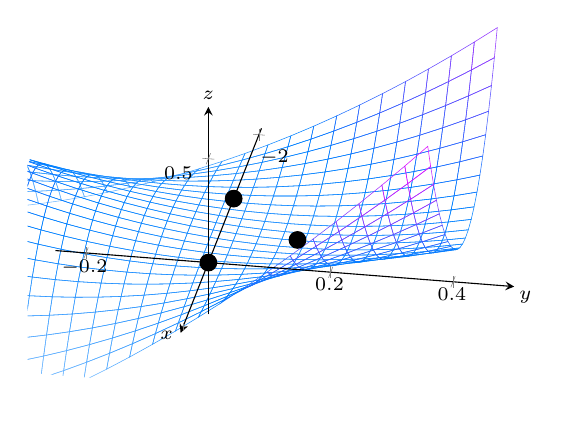
\begin{tikzpicture}
        \begin{axis}%
          [tick label style={font=\scriptsize},axis on top,
	    axis lines=center,
	    view={100}{45},
	    name=myplot,
	    %xtick=\empty,
	    %ytick={5},
	    %ztick={.7,-.7},
	    minor xtick=1,
	    minor ytick=1,
	    ymin=-.25,ymax=.5,
	    xmin=-2.1,xmax=1.1,
	    zmin=-.25, zmax=.75,
	    every axis x label/.style={at={(axis cs:\pgfkeysvalueof{/pgfplots/xmax},0,0)},xshift=-5pt,yshift=-1pt},
	    xlabel={\scriptsize $x$},
	    every axis y label/.style={at={(axis cs:0,\pgfkeysvalueof{/pgfplots/ymax},0)},xshift=4pt,yshift=-4pt},
	    ylabel={\scriptsize $y$},
	    every axis z label/.style={at={(axis cs:0,0,\pgfkeysvalueof{/pgfplots/zmax})},xshift=0pt,yshift=4pt},
	    zlabel={\scriptsize $z$},colormap/cool
	  ]
          
          \addplot3[domain=-1.75:1,,y domain=-.5:.4,mesh,samples=25,samples y=25,very thin,z buffer=sort] {x^2*y+x*y+y^2};
          
          
          \filldraw [black,] (axis cs:-1,0,0) circle (3pt);
          \filldraw [black,] (axis cs:0,0,0) circle (3pt);
          \filldraw [black,] (axis cs:-.5,.125,-.016) circle (3pt);
          
        \end{axis}
      \end{tikzpicture}
    \end{image}
    Note how this function does not vary much near the critical
    points. Visually it is difficult to determine whether a point is a
    saddle point or local minimum (or even a critical point at
    all!). This is one reason why the second derivative test is so
    important to have.
  \end{explanation}
\end{example}

For some interesting extra reading check out:
\begin{itemize}
\item \link[\textit{Three Observations on a Theme: Editorial Note}, D.A.\ Smith, Mathematics Magazine, May 1985]{http://www.jstor.org/stable/2689908}.
\item \link[\textit{A Surface with One Local Minimum}, J.M.\ Ash and H.\ Sexton, Mathematics Magazine, May 1985]{http://www.jstor.org/stable/2689909}.
\item \link[\textit{``The Only Critical Point in Town'' Test}, I.\ Rosenholtz and  L.\ Smylie, Mathematics Magazine, May 1985]{http://www.jstor.org/stable/2689910}.
\item \link[\textit{Two Mountains Without a Valley}, I.\ Rosenholtz, Mathematics Magazine, February 1987]{http://www.jstor.org/stable/2690137?seq=10}.
\end{itemize}
  
\end{document}
